\def\year{2019}\relax
\documentclass[letterpaper]{article} % DO NOT CHANGE THIS
\usepackage{aaai19}  % DO NOT CHANGE THIS
\usepackage{times}  % DO NOT CHANGE THIS
\usepackage{helvet} % DO NOT CHANGE THIS
\usepackage{courier}  % DO NOT CHANGE THIS
\usepackage[hyphens]{url}  % DO NOT CHANGE THIS
\usepackage{graphicx} % DO NOT CHANGE THIS
\urlstyle{rm} % DO NOT CHANGE THIS
\def\UrlFont{\rm}  % DO NOT CHANGE THIS
\usepackage{graphicx}  % DO NOT CHANGE THIS
\frenchspacing  % DO NOT CHANGE THIS
\setlength{\pdfpagewidth}{8.5in}  % DO NOT CHANGE THIS
\setlength{\pdfpageheight}{11in}  % DO NOT CHANGE THIS
\nocopyright
\graphicspath{{images/}}
%PDF Info Is REQUIRED.
% For /Author, add all authors within the parentheses, separated by commas. No accents or commands.
% For /Title, add Title in Mixed Case. No accents or commands. Retain the parentheses.
\pdfinfo{
/Title (Enhancing Images with Deep Convolutional Generative Adversarial Networks)
/Author (Mark Wesley Harris)
} %Leave this	
% /Title ()
% Put your actual complete title (no codes, scripts, shortcuts, or LaTeX commands) within the parentheses in mixed case
% Leave the space between \Title and the beginning parenthesis alone
% /Author ()
% Put your actual complete list of authors (no codes, scripts, shortcuts, or LaTeX commands) within the parentheses in mixed case. 
% Each author should be only by a comma. If the name contains accents, remove them. If there are any LaTeX commands, 
% remove them. 

% DISALLOWED PACKAGES
% \usepackage{authblk} -- This package is specifically forbidden
% \usepackage{balance} -- This package is specifically forbidden
% \usepackage{caption} -- This package is specifically forbidden
% \usepackage{color (if used in text)
% \usepackage{CJK} -- This package is specifically forbidden
% \usepackage{float} -- This package is specifically forbidden
% \usepackage{flushend} -- This package is specifically forbidden
% \usepackage{fontenc} -- This package is specifically forbidden
% \usepackage{fullpage} -- This package is specifically forbidden
% \usepackage{geometry} -- This package is specifically forbidden
% \usepackage{grffile} -- This package is specifically forbidden
% \usepackage{hyperref} -- This package is specifically forbidden
% \usepackage{navigator} -- This package is specifically forbidden
% (or any other package that embeds links such as navigator or hyperref)
% \indentfirst} -- This package is specifically forbidden
% \layout} -- This package is specifically forbidden
% \multicol} -- This package is specifically forbidden
% \nameref} -- This package is specifically forbidden
% \natbib} -- This package is specifically forbidden -- use the following workaround:
% \usepackage{savetrees} -- This package is specifically forbidden
% \usepackage{setspace} -- This package is specifically forbidden
% \usepackage{stfloats} -- This package is specifically forbidden
% \usepackage{tabu} -- This package is specifically forbidden
% \usepackage{titlesec} -- This package is specifically forbidden
% \usepackage{tocbibind} -- This package is specifically forbidden
% \usepackage{ulem} -- This package is specifically forbidden
% \usepackage{wrapfig} -- This package is specifically forbidden
% DISALLOWED COMMANDS
% \nocopyright -- Your paper will not be published if you use this command
% \addtolength -- This command may not be used
% \balance -- This command may not be used
% \baselinestretch -- Your paper will not be published if you use this command
% \clearpage -- No page breaks of any kind may be used for the final version of your paper
% \columnsep -- This command may not be used
% \newpage -- No page breaks of any kind may be used for the final version of your paper
% \pagebreak -- No page breaks of any kind may be used for the final version of your paperr
% \pagestyle -- This command may not be used
% \tiny -- This is not an acceptable font size.
% \vspace{- -- No negative value may be used in proximity of a caption, figure, table, section, subsection, subsubsection, or reference
% \vskip{- -- No negative value may be used to alter spacing above or below a caption, figure, table, section, subsection, subsubsection, or reference

\setcounter{secnumdepth}{0} %May be changed to 1 or 2 if section numbers are desired.

% The file aaai19.sty is the style file for AAAI Press 
% proceedings, working notes, and technical reports.
%
\setlength\titlebox{2.5in} % If your paper contains an overfull \vbox too high warning at the beginning of the document, use this
% command to correct it. You may not alter the value below 2.5 in
\title{Enhancing Images with Deep Convolutional Generative Adversarial Networks}
%Your title must be in mixed case, not sentence case. 
% That means all verbs (including short verbs like be, is, using,and go), 
% nouns, adverbs, adjectives should be capitalized, including both words in hyphenated terms, while
% articles, conjunctions, and prepositions are lower case unless they
% directly follow a colon or long dash
\author{Mark Wesley Harris\\ % All authors must be in the same font size and format. Use \Large and \textbf to achieve this result when breaking a line
% If you have multiple authors and multiple affiliations
% use superscripts in text and roman font to identify them. For example, Sunil Issar,\textsuperscript{\rm 2} J. Scott Penberthy\textsuperscript{\rm 3} George Ferguson,\textsuperscript{\rm 4} Hans Guesgen\textsuperscript{\rm 5}. Note that the comma should be placed BEFORE the superscript for optimum readability
University of Colorado Colorado Springs\\
wharris2@uccs.edu % email address must be in roman text type, not monospace or sans serif
}
\begin{document}

\maketitle

\begin{abstract}
Abstract.
\end{abstract}

\section{Introduction}
\label{sec:introduction}
Rendering full-length feature films is burdensome for current technologies.
Rendering a single frame of an animation is highly dependent upon the rendering software
and scene complexity,
but for the most part the rendering process is completely dependent upon the renderer.
There are no shortcuts to be made.

This research is focused on studying how to generate renderings for animations using
Machine Learning.

\section{Related Work}
\label{sec:related_work}
The Generative Adversarial Network (GAN) was first proposed by
\cite{generative_adversarial_networks}
as a way to
train a model to produce more realistic images. The network is made up of two architectures:
a generator, G, and a disciminator, D.

The Deep Convolutional Generative Adversarial Network (DCGAN) was first proposed by
\cite{unsupervised_learning}. The architecture is similar to a GAN,
but uses convolutional and convolutional-transpose layers in D and G, respectively.

\section{Proposed Work}
\label{sec:proposed_work}
Foundational example DCGAN repository titled ``Deep Convolution Generative Adversarial Networks''
, created by Pytorch \cite{dcgan_git}. This repository is explained in a walkthrough
by Pytorch \cite{dcgan_example}.

\subsection{Dataset Creation}
\label{subsec:data}
Create a dataset of 10,000 32 x 32 pixel images based off of previous research.
Images are blurred and small anomolies are added.
The original images are kept to form an image pair with the altered images.

\begin{figure}[htbp]
\centerline{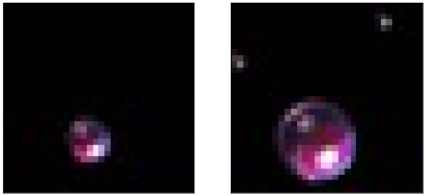
\includegraphics[width=8cm]{training_pair.png}}
\caption{Example of input (left) and expected output (right).}
\label{fig:training_pair}
\end{figure}

\subsection{Model Construction}
\label{subsec:model}

\section{Evaluation}
\label{sec:methods/evaluation}
The architecture will be evaluated on how well it is able to learn how to
enhance an altered image. After optimization and training has taken place,
an unknown altered image will be input into the algorithm, and the output
will be compared to the original, unaltered image.

\section{Conclusion}
\label{sec:conclusion}

\cite{3D_capsule_networks}
\cite{combining_multiple_cnn}
\cite{conditional_image_generation}
\cite{deep_video_prediction}
\cite{fusionnet}
\cite{generative_adversarial_networks}
\cite{image_to_image}
\cite{show_and_tell}
\cite{pixelcnn++}
\cite{pose_cnn}
\cite{pose_guided_image_generation}
\cite{unsupervised_learning}
\cite{dcgan_git}

\bibliography{proposal}
\bibliographystyle{aaai}

\end{document}
